\documentclass[a4paper,12pt]{report}
\usepackage[latin1]{inputenc}
\usepackage[T1]{fontenc}
\usepackage[english]{babel}
\usepackage{float}
\usepackage{hyperref}
\usepackage{listings}
\usepackage{cite}
\usepackage{acro}
\usepackage{graphicx}
\usepackage[nodayofweek]{datetime}

\DeclareGraphicsRule{*}{mps}{*}{}

% Commands
\newcommand{\HRule}{\rule{\linewidth}{0.5mm}} % Defines a new command for the horizontal lines

\begin{document}

	\begin{titlepage}
		\begin{centering}
		 
		%	HEADING SECTIONS
		
		\textsc{\textbf{\LARGE{Industrial Visit Report}}}\\[0.5cm]

		\textbf{\textit{\large{A Project Report}}}\\[1.5cm]

		\large{submitted in partial fulfilment for the award of the degree of Bachelor of Technology in Computer Science and Engineering}\\[1.5cm]

		\large{by}\\[0.5cm]

		\textbf{Kevin Joseph     }\\
		{13400032 S7 R}\\[2cm]
		

		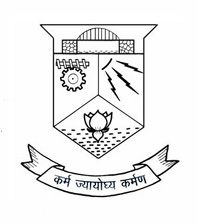
\includegraphics[width=5cm]{images/logo.jpg}

		\textsc{Department of Computer Science and Engineering}\\
		\textsc{College of Engineering Trivandrum}\\
		\textsc{Kerala}\\[0.5cm]
		\textsc{May 2017}\\
		\vfill % Fill the rest of the page with whitespace
		\end{centering}
	\end{titlepage}

	\begin{titlepage}
		\begin{centering}
			\textsc{\large{Department of Computer Science and Engineering}}\\
			\textsc{\large{College of Engineering Trivandrum}}\\[0.5cm]

			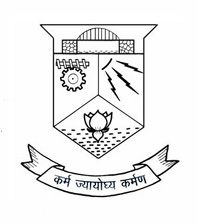
\includegraphics[width=5cm]{images/logo.jpg}\\[0.5cm]
			\textbf{\textit{\LARGE\textsc{{certificate}}}}\\[0.3cm]

		\end{centering}

		\begin{sloppypar}
		\large{This is to certify that this Industrial visit report is a bonafide record of the industrial visits undergone by Kevin Joseph (13400032), under our guidance towards partial fulfillment of the requirements for the award of Degree of bachelor of Technology in Computer Science and Engineering of the University of Kerala during the year 2016}\\[1.5cm]
		\end{sloppypar}

		\begin{minipage}{0.4\textwidth}
		\begin{flushleft}
		\begin{centering} \large
		\large{Mr. Sreelal S}\\
		\small{\textit{\textbf{Dept. of Computer Science and Engineering}}}\\[1.5cm]

		\end{centering}
		
		\end{flushleft}
		\end{minipage}
		~
		\begin{minipage}{0.5\textwidth}
		\begin{centering} \large
			\large{Mrs. Liji P I}\\
			\small{\textit{\textbf{Head of Department}}}\\
			\small{\textit{\textbf{Dept. of Computer Science and Engineering}}}\\
		\end{centering}
		\end{minipage}\\[1.0cm]

		\begin{flushleft}
		Place: Trivandrum\\
		Date:  11-05-2017\\
		\end{flushleft}
		\vfill % Fill the rest of the page with whitespace
	\end{titlepage}

	% TODO Ack before this
	\pagenumbering{roman}
	
	\newpage
	\tableofcontents
	\newpage

	\pagenumbering{arabic}
	\chapter{Sensomate Systems}
		\section{About The Company}
		We visited Sensomate Systems on 21st January 2016. Sensomate Systems is a startup based in trivandrum with its office inside technopark (PHASE 1). We visited their office and were introduced to the work done by them and a overview of their products and software developement process. Sensomate is a company in the starup phase, but has had visible and continious growth in the previous years. They now have offices in Trivandrum, Chennai, Banglore, Canada and Saudi Arabia and clients across the world. The Company CEO is Krishnendu Gopalakrishnan and their team consists of 15 developers, 4 testers, 2 architects and 2 UX engineers.  
		\begin{figure}[!ht]
					\begin{centering}
						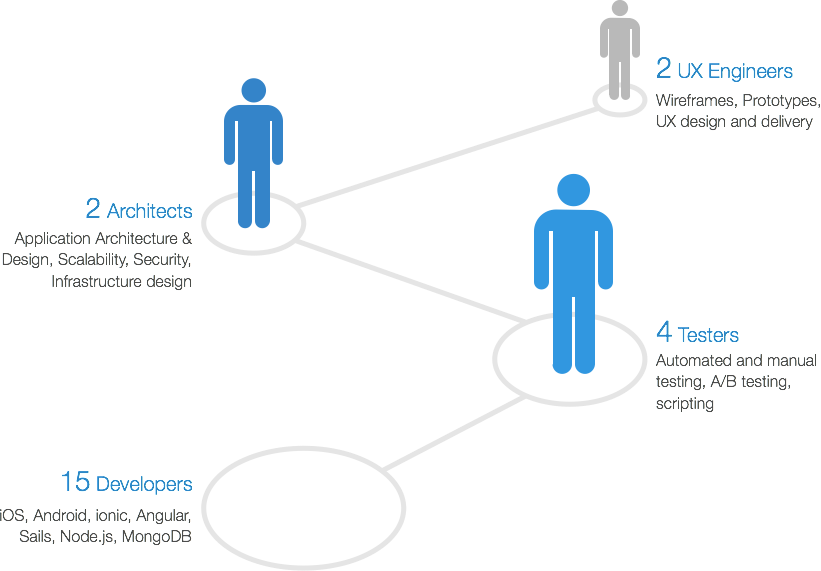
\includegraphics[width=10cm]{images/team.png}\\
					\end{centering}
				\end{figure}
		Their mission is: ``Enchanting our customers, employees and shareholders by creating cutting edge and value add technology products and solutions that touches and leaves a lasting impression on how the world works and live.''
			\subsection{Technopark}
			Sensomate Systems is based in trivandrum, inside Technopark. Technopark is a technology park in Thiruvananthapuram, Kerala, India. It is the largest Information Technology park in Asia in terms of built up area. The park is dedicated to IT ventures. Launched in 1990, Technopark as of 2015 has 9.33 million square feet of built-up area, and is home to over 350 companies, employing nearly 60,000 professionals. Technopark is currently on an expansion mode by adding another 37 hectares as part of Phase III expansion and 423 acres as Technocity-an integrated IT township near Pallippuram. The policy of economic liberalisation initiated by the government of India in 1991 and the rapid growth of the global software industry during the 1990s substantially contributed to its growth. During the global financial crisis of 2007-2010, the park saw a period of reduced growth in 2009-10, where the exports recorded was only 2.8\% more than the previous year. As of 2017, Technopark accounts for about 70\% of IT exports from Kerala, which was 80\% in 2014.
			The units in Technopark include domestic firms, joint ventures and subsidiaries of foreign companies engaged in a wide variety of activities, which include embedded software development, smart card technology, enterprise resource planning (ERP), process control software design, engineering and computer-aided design software development, IT Enabled Services (ITES), process re-engineering, animation and e-business. Technopark is owned and administered by the Government of Kerala and is headed by a chief executive officer. In addition to this, it has a Governing Council and a Project Implementation Board, both of which include top officials of the government.[5] Administrative offices, including that of the CEO, are housed in the Park Centre building. Technopark also hosts a Technology Business Incubation Cell under Kerala Startup Mission.
		\newpage
		\section{Products}
			\subsection{Proximity Beacons}
			Sensomate systems provides Bluetooth Low Energy(BLE) based proximity beacons separately and their also used in their other products like attendance system and schoolsafe.
			\subsection{Attendance System}
			The above mentiioned proximity beacons can be used in an attendance and asset management system when clubbed with an interface and and bluetooth sensor devices. For the sensor side devices they used small android based devices to sense beacons and transmit data about them to a central server. The data on the central server is used to generate realtime statistics on an interface to be managed by a manager or group of managers.
			\subsection{Indoor Navigation System}
			Indoor navigation System is also based on the BLE beacons. Usually we use GPS for navigation, but a GPS on our smartphones can only give us an accuracy of upto 7-10m. This is not enough to navigate an indoor space, hence they used proximity beacons. The proximity beacons are used to mark places in an indoor space and the users' devices show position on an app. based on the beacons that they can sense. If the beacons are placed carefully, it is possible to attain a pretty good navigation system. The mention app is also developed by Sensomate as a part of this product.
			\subsection{SchoolSafe}
			This product was inspired by the problem of children missis stops of getting missed out in school busses in Saudi Arabia. The solution was to have proximity beacons attatched to school id card and to track children in real time in busses and schools. this allows the system to send alerts to concerned people in case of unusual occurences and also provides a way to manage attendance. The main features include bus tracking, attendance management, parent teacher apps, context aware alerts etc.   
		\section{Software Development Lifecycle and Timeline}
		\section{Topics Discussed}
			\subsection{Data Analytics}
			\subsection{Realtime Web}
			\subsection{Mobile Application}
			\subsection{Internet of Things}
			\subsection{Content Managemant Systems}
			\subsection{Cloud Computing}
	
\end{document}